\documentclass[pdf]{beamer}
\mode<presentation>{} 

\usepackage{tabularx}
\usepackage{hyperref}
\usepackage{pgf}
\usepackage{tikz}
\usetikzlibrary{trees}
\usetikzlibrary{arrows,automata}
\usetikzlibrary{automata,positioning}
\usetikzlibrary{shapes}
\usepackage{tikz-qtree,tikz-qtree-compat}
\usepackage{mathtools,enumerate,amssymb}
\usepackage[utf8]{inputenc}
\usepackage[T1]{fontenc}
\usepackage{wrapfig}
\usepackage{setspace}
\usepackage{bbding}
\usepackage{adjustbox}

\definecolor{ballblue}{rgb}{0.13, 0.67, 0.8}

\title{Teoria traducerii}
\subtitle{Limbaje formale şi translatoare (Compilatoare)}
\AtBeginSection[]{}

\setbeamertemplate{sidebar right}{}
\setbeamertemplate{footline}{%
\hfill\usebeamertemplate***{navigation symbols}
\hspace{1cm}\insertframenumber{}/\inserttotalframenumber}

\begin{document}



\begin{frame}
	\titlepage
	
\begin{flushright}
Mihai-Lica Pura\\
\end{flushright}

\end{frame}



\begin{frame}{Cuprins}
\begin{itemize}
\item
Definiția unui compilator/translator
\item
Clasificarea compilatoarelor
\item
Etapele traducerii
\item
Proiectarea compilatoarelor

\end{itemize}
\end{frame}



\begin{frame}{Definiţii}
\begin{itemize}
\item
\textbf{Compilator/Translator} - programul sau setul de programe care traduce propoziţii scrise într-un limbaj (\textbf{limbajul sursă}) într-un alt limbaj (\textbf{limbajul ţintă})

\begin{figure}
\centering
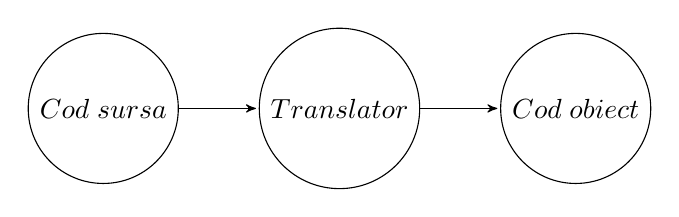
\begin{tikzpicture}[>=stealth',shorten >=1pt,auto,node distance=3cm]

  \node[state] (q0)      {$Cod \; sursa$};
  \node[state]         (q1) [right of=q0]  {$Translator$};
  \node[state]         (q2) [right  of=q1] {$Cod \; obiect$};
  \path[->] (q0)  edge node {} (q1)
		(q1) edge node {} (q2);

\end{tikzpicture}
\end{figure}

\begin{itemize}
\item
propoziția de intrare - \textbf{cod sursă}
\item
propoziția de ieşire - \textbf{cod obiect}
\end{itemize}
\end{itemize}
\end{frame}



\begin{frame}{Definiţii}
\begin{itemize}
\item
motivul cel mai des întâlnit pentru care este nevoie de traducerea codului sursă constă în nevoia de a crea un \textbf{program executabil}.
\item
termenul \textbf{compilator} se foloseşte în special pentru programele care traduc:

\begin{itemize}
\item
cod sursă scris într-un \textbf{limbaj de programare de nivel înalt}
\item
în cod obiect într-un \textbf{limbaj de programare nivel scăzut} (limbaj maşină)
\end{itemize}
\end{itemize}
\end{frame}



\begin{frame}{Definiţii}
\begin{itemize}
\item
\textbf{decompilator (decompiler)} - programul care poate să traducă dintr-un limbaj de nivel scăzut într-un limbaj de nivel înalt
\item
\textbf{translator de limbaje, translator sursă la sursă sau convertor de limbaje} - program capabil să facă traduceri între două limbaje de programare de nivel înalt
\item
\textbf{rescriitor de limbaj (rewriter)} - program care poate schimba forma de exprimare a codului sursă, fără a schimba limbajul în care a fost scris
\end{itemize}
\end{frame}



\begin{frame}{Clasificarea compilatoarelor}
după \textbf{platforma ţintă} (platforma pe care va fi executat codul obiect produs de către compilator):

\begin{itemize}
\item
\textbf{Compilatoare native (native/hosted compilers)}

\begin{itemize}
\item
codul obiect va fi rulat pe acelaşi tip de mașină şi pe acelaşi tip de sistem de operare ca şi cele pe care a fost rulat compilatorul
\newline
Ex: compilatorul din Microsoft Visual Studio 2017
\end{itemize}
\end{itemize}
\end{frame}



\begin{frame}{Clasificarea compilatoarelor}
\begin{itemize}
\item
\textbf{Cross compiler}

\begin{itemize}
\item
codul obiect generat de către compilator va fi rulat pe un alt tip de platformă

\item
acest tip de compilatoare se utilizează în special pentru dezvoltarea de programe pentru sistemele embedded, care nu au fost proiectate astfel încât să suporte un mediu de dezvoltare
\newline
Ex: programele pentru microprocesoare\newline
\end{itemize}

\item
Ieşirea compilatorului care produce cod obiect pentru o maşină virtuală poate fi executat atât pe acelaşi tip de platformă ca şi cea pe care a rulat compilatorul, cât şi pe un alt tip. De aceea, aceste compilatoare nu sunt clasificate ca şi native sau cross.
\end{itemize}
\end{frame}



\begin{frame}{Etapele traducerii}
\begin{itemize}
\item
\textbf{1) Analiza lexicală}
\begin{itemize}
\item
pe baza: gramaticii regulare care definește sintaxa tipurilor de atomi lexicali

\item
intrare - codul sursa (secvența de caractere)

\item
ieșire - secvența de atomi lexicali 
\end{itemize}

\item
\textbf{2) Analiza sintactică}
\begin{itemize}
\item
pe baza: gramaticii independente de context care definește sintaxa propozițiilor limbajului

\item
intrare - secvența de atomi lexicali

\item
ieșire - arborele sintactic (și tabela de simboli)
\end{itemize}

\item
\textbf{3) Analiza semantică}
\end{itemize}
\end{frame}



\begin{frame}{Etapele traducerii}
\begin{itemize}
\item
\textbf{4) Translatare in cod intermediar}
\begin{itemize}
\item
intrare - arborele sintactic

\item
ieșire - codul intermediar
\end{itemize}

\item
\textbf{5) Optimizarea codului intermediar}
\begin{itemize}
\item
intrare - codul intermediar

\item
ieșire - codul intermediar optimizat
\end{itemize}

\item
\begin{itemize}
\item
Optiune 1) \textbf{Generarea de cod} 
\begin{itemize}
\item
ingtrare - codul intermediar optimizat

\item
ieșire - fișierul executabil (cod mașină)
\end{itemize}

\item
Optiune 2) \textbf{Interpretarea}
\begin{itemize}
\item
simularea execuției codului intermediar de catre un interpretor
\end{itemize}
\end{itemize}
\end{itemize}
\end{frame}



\begin{frame}{Etapele traducerii exemplificate pentru o propoziţie în limbaj natural}
\begin{figure}
\centering
    \scalebox{0.7}{
\begin{tabular}{| p{2cm} | p{3cm} | p{3cm} | p{3cm} |}
	\hline
	& Propozitia este valida din punct de vedere lexical? (\textbf{atomii lexicali care compun propozitia apartin vocabularului limbajului}?)& Propozitia este corecta din	punct de vedere sintactic? (\textbf{atomii lexicali sunt in ordinea corecta}?)  & Propozitia este corecta din punct de vedere semnantic? (\textbf{propozitia are inteles}?) \\\hline
	Eminescu este un scriicotr. & NU & & \\ \hline
	Eminescu scriitor un este. & DA & NU & \\ \hline
	Scriitor este un Eminescu. & DA & DA & NU \\ \hline
	Eminescu este un scriitor. & DA & DA & DA \\ \hline
\end{tabular}
}
\end{figure}
\end{frame}



\begin{frame}{Etapele traducerii exemplificate pentru o propoziţie în limbaj de programare}

\  $  \ a \  = \  b \ + \ c \  * \  d \ $
\newline\centering$\downarrow$

\hfill{\framebox[80pt][c]{Analizor lexical} $\leftarrow$ \framebox[30pt]{flex} $\leftarrow$ patterns (.l)}
\\[15pt]


\ $ id1 \ = \ id2 \ + \ id3 \ * \ id4$
\newline\centering$\downarrow$

\hfill\framebox[80pt][c]{Analizor sintactic} $\leftarrow$ \framebox[30pt]{bison} $\leftarrow$ grammar (.y)
\newline\centering$\downarrow$
\end{frame}



\begin{frame}{Etapele traducerii exemplificate pentru o propoziţie în limbaj de programare}
\begin{figure}[h!]
\centering
\begin{tikzpicture}
\node {$=$}
child {node {id1}}
child {node {$+$}
	child {node{id2}}
	child {node{$*$}   child{node{id3}}   child{node{id4}}}
};
\end{tikzpicture}
\end{figure}

\centering$\downarrow$
\end{frame}



\begin{frame}{Etapele traducerii exemplificate pentru o propoziţie în limbaj de programare}
\begin{center}
load \- \- \- \- \- \- \- id3 
\newline
mul \- \- \- \- \- \- \- \-  id4
\newline
add \- \- \- \- \- \- \- \-  id2
\newline
store  \- \- \- \- \-  \- \- id1
\newline
\end{center}
\end{frame}



\begin{frame}{Proiectarea compilatoarelor}
\begin{itemize}
\item
\textbf{Abodarea monolitică}

\begin{itemize}
\item
compilator care traduce un limbaj relativ simplu
\item
este scris de catre o singura persoana
\end{itemize}

\item
\textbf{Abordarea modulară}

\begin{itemize}
\item
limbajul de tradus este complex
\item
calitatea codului obiect generat trebuie sa fie maximă
\item
dezvoltarea compilatorului va fi împărițită la mai multe persoane care lucreaza în paralel
\item
este mult mai ușor să se înlocuiasca un modul component cu o implementare mai bună
\item
sau sa se adauge ulterior alte module
\item
subiectul unui concurs lansat de Production Quality Compiler-Compiler Project (PQCC) al Universității Carnegie Mellon
\end{itemize}
\end{itemize}
\end{frame}



\begin{frame}{Proiectare compilatoarelor}
\textbf{Abordarea modulară}
\begin{itemize}
\item
\textbf{front-end} (partea "din față" a unui compilator)

\begin{itemize}
\item
analizează codul sursă cu scopul de a construi o reprezentare internă a acestuia \textbf{reprezentarea intermediară} - (de nivel mai scazut decat cel al limbajului in care a fost scris codul sursă)
\item
crează, populează și gestionează \textbf{tabela de simboli}

\begin{itemize}
\item
o structura de date care memorează pentru fiecare atom lexical informațiile semantice asociate
\end{itemize}

\end{itemize}

\item
\textbf{back-end} (partea "din spate" a compilatorului)

\begin{itemize}
\item
analize, transformări și optimizari specifice pentru o anumită platformă
\item
generarea de cod pentru un anumit sistem de operare și pentru un anumit procesor
\end{itemize}
\end{itemize}
\end{frame}



\begin{frame}{Front-end}
\textbf{Etape:}
\begin{itemize}
\item 
1. \textbf{reconstruirea liniilor}
\item
2. \textbf{analiza lexicală}
\item
3. \textbf{preprocesarea}
\item
4. \textbf{analiza sintactică}
\item
5. \textbf{analiza semantică}
\item
6. \textbf{generearea codului intermediar}
\end{itemize}
\end{frame}



\begin{frame}{Back-end }
\textbf{Etape:}
\begin{itemize}
\item
1. \textbf{analiza codului intermediar}
\item
2. \textbf{optimizarea codului intermediar}
\item
3. \textbf{generarea codului final}
\end{itemize}
\end{frame}



\begin{frame}{Reconstruirea liniilor}
\begin{itemize}
\item
pregăteşte codul sursă pentru analiza gramaticală, convertind secvenţa de caractere într-o formă canonică

\item
necesară în cazul limbajelor în care 
\begin{itemize}
\item
cuvintele cheie sunt marcate prin simboli speciali (\textbf{stropping})
\item
se permite prezenţa în cadrul identificatorilor a unui număr arbitrar de spaţii
\end{itemize}
\end{itemize}
\end{frame}



\begin{frame}{Reconstruirea liniilor}
\begin{itemize}
\item
\textbf{stropping} refers to the method used to mark letter sequences as having a special property (most often being a keyword or certain type of variable/storage location)

\begin{itemize}
\item
în limbajul Algol68 cuvintele cheie sunt marcate prin prefixarea cu un apostrof: 'BEGIN
\item
în limbajul Algol60 cuvintele cheie sunt marcate prin scrierea lor între apostrofi: 'BEGIN'
\item
limbajele Ruby şi Pearl utilizează caracterere sigil pentru a identifica caracteristicile unei variabile/constante
\end{itemize}

\item
stropping oferă posibilitatea de a utiliza \textbf{aceeaşi secvenţă de caractere pentru a reprezenta atomi lexicali cu semnificaţie diferită}

\end{itemize}
\end{frame}



\begin{frame}{Reconstruirea liniilor}
\begin{itemize}
\item
\textbf{PHP} (largely inspired by Perl)
\begin{itemize}
\item
any name preceded by \$ is a variable name
\item
names not prefixed by this are considered constants or functions
\end{itemize}

\item
\textbf{Ruby}
\begin{itemize}
\item
ordinary variables lack sigils
\item
\$ is prefixed to global variables
\item
@ is prefixed to instance variables
\item
@@ is prefixed to class variables 
\end{itemize}

\item
\textbf{Windows PowerShell}
\begin{itemize}
\item
variable names are prefixed by the \$ sigil
\end{itemize}
\end{itemize}
\end{frame}



\begin{frame}{Reconstruirea liniilor}
\begin{itemize}
\item
\textbf{Transact-SQL}
\begin{itemize}
\item
@ precedes a local variable or parameter name
\item
@@ prefix distinguishes system variables (known as global variables)
\end{itemize}

\item
\textbf{C\#}
\begin{itemize}
\item
any variable names may be prefixed with @ to allow the use of variable names that would otherwise conflict with keywords
\item
when @ sigil is applied to string literals it changes the way they are interpreted (character escapes are not used and strings can extend over multiple lines)
\end{itemize}
\end{itemize}
\end{frame}



\begin{frame}{Analiza lexicală}
\begin{itemize}
\item
\textbf{împarte codul sursă în atomi lexicali} - pe baza gramaticii regulare care definește sintaxa tipurilor de atomi lexicali
\newline

\item
\textbf{extrage informaţii privind locaţia în codul sursă} a fiecărui atom lexical (linie și coloană)
\newline

\item
detectează \textbf{atomii lexicali care nu aparţin limbajului} respectiv

\end{itemize}
\end{frame}



\begin{frame}{Analiza lexicală}
\begin{itemize}
\item
un atom lexical (token) este o componentă singulară indivizibilă a unui limbaj - unitate lexicală

\item
scopul analizei lexicale este \textbf{transformarea şirului de caractere care formează codul sursă într-o secvenţă de atomi lexicali}

\item
dacă lipseşte etapa de reconstrucţie a liniilor, analizorul lexical trebuie să elimine şi separatorii din codul sursă

\item
poate \textbf{elimina comentariile} din codul sursă, caz în care operaţia respectivă nu va mai trebui realizată în etapa de preprocesare
\end{itemize}
\end{frame}



\begin{frame}{Tipuri de atomi lexicali}
\begin{enumerate}
	\item
	\textbf{Cuvintele rezervate}
	\\
	Ex:
	\begin{enumerate}[a) ]
		\item
		C: int, long, float, double, unsigned, void, if, else, for, while, do, switch, default, case, struct
		\item
		C++: class, inline, virtual
	\end{enumerate}	
	
	\item
	\textbf{Identificatorii}
	\begin{enumerate}[a) ]
		\item
		nume de variabile, de constante, de funcții, de structuri/clase, de namespace-uri, etc.
	\end{enumerate}
	
	\item
	\textbf{Constante }
	\\
	Ex:
	\begin{enumerate}[a) ]
		\item
		intregi: (12, +3, 0)
		\item
		reale (12.0, +3.2, 0.0)
		\item
		caracter ('a', '\textbackslash n')
		\item
		şir de caractere ("", "la facultate")
		\item
		bool (true, false)
		\item
		hexazecimale (0x45, 0xFA)
		\item
		ș.a.
	\end{enumerate}
\end{enumerate}
\end{frame}



\begin{frame}{Tipuri de atomi lexicali}
\begin{enumerate}
	\item[4.]
	\textbf{Operatori }
	\begin{enumerate}[A. ]
		\item
		aritmetici
		\\
		Ex: C: +,-,*,/,\%
		\item
		logici
		\\
		Ex: C: \&,|,!
	\end{enumerate}
	
	\item[5.]
	\textbf{Semne de punctuaţie }(simboli sau grupuri de simboli cu rol delimitativ)
	\\
	Ex: C: spaţiu, punct şi virgulă
	
	\item[6.]
	\textbf{Comentariile}
	\\
	Ex: C: liniile care încep cu //, sau şirurile de caractere dintre "/*" şi "*/"
\end{enumerate}
\end{frame}



\begin{frame}{Analiza lexicală}
\begin{itemize}
\item
fiecare atom lexical este caracterizat prin doua elemente
\begin{itemize}
\item
\textbf{tipul}

\begin{itemize}
\item
necesar în analiza sintactică

\item
este dat de clasa de atomi lexicali din care face parte
\end{itemize}


\item
\textbf{valoarea semantică}
\begin{itemize}
\item
necesară în analiza semantică

\item
este reprezentata de succesiunea de caractere care formeaza atomul lexical respectiv
\end{itemize}
\end{itemize}

\item
Ex: identificator, NumeVariabila
\end{itemize}
\end{frame}



\begin{frame}{Analiza lexicală}
\begin{itemize}
\item
împărțirea se bazeaza pe faptul că în \textbf{analiza sintactică nu este important care atom lexical urmează, ci mai ales ce tip de atom lexical urmează}

\item
\textbf{exact care atom lexical a urmat va fi important în analiza semantică}

\item
Ex: pentru instrucțiunea "int a1;"
\begin{itemize}
\item
la analiza sintactică este important că după cuvântul cheie "int" urmează un identificator
\item
nu are importanță că acest identificator este "a1"
\item
iar la analiza semnatică va fi nevoie și de informația cum că identificatorul respectiv este chiar "a1"
\end{itemize}
\end{itemize}
\end{frame}



\begin{frame}{Implementarea analizorului lexical}
\begin{itemize}
\item 
analiza lexicală este \textbf{partea cea mai critică pentru un compilator, din punct de vedere al performanţelor}

\item
de exemplu, dacă analizorul lexical este implementat în forma comandată de către analizorul sintactic, atunci el va fi apelat pentru fiecare atom lexical din codul sursă

\item
rezultă deci că această componentă trebuie să fie foarte eficientă

\item 
căutarea liniară sau utilizarea unei succesiuni foarte lungi de instrucţiuni \textit{if} la procesarea unui atom lexical trebuie evitate
\end{itemize}
\end{frame}



\begin{frame}{Implementarea analizorului lexical}
\begin{itemize}
\item
analizorul lexical ar trebui să ofere şi
\begin{itemize}
\item
o bună \textbf{diagnosticare a erorilor} care survin la analiză
\item
un \textbf{mecanism eficient de tratare} a acestora
\end{itemize}

\item
Ex:
\begin{itemize}
\item
dacă a fost folosită o constantă numerică cu valoarea mai mare decât valoarea maximă acceptată de către limbaj, atunci:
\begin{itemize}
\item
analizorul lexical ar trebui să emită un mesaj în acest sens
\item
şi să înlocuiască valoarea constantei cu valoarea maximă
\end{itemize}

\item
dacă a fost folosit un şir de caractere cu o lungime mai mare decât lungimea maximă acceptată, atunci:
\begin{itemize}
\item
analizorul lexical trebuie să emită un mesaj în acest sens
\item
şi să trunchieze şirul la lungimea maximă acceptată
\end{itemize}
\end{itemize}
\end{itemize}
\end{frame}



\begin{frame}{Implementarea analizorului lexical}
\begin{itemize}
\item
în vederea generării de mesaje de eroare sau de atenţionare cât mai utile:
\begin{itemize}
\item
analizorul lexical trebuie \textbf{să extragă şi informaţii privind locaţia în codul sursă} a fiecărui atom lexical
\item
acestea vor fi folosite nu numai pentru mesajele rezultate în urma analizei lexicale, ci și pentru cele de la analiza sintactică și semantică
\end{itemize}
\end{itemize}
\end{frame}



\begin{frame}{Implementarea analizorului lexical}
\begin{itemize}
\item
a scrie un analizor lexical înseamnă a scrie un program care este capabil să recunoască şi să extragă toate cuvintele (secvenţele de caractere) care aparţin limbajului supus analizei

\item
fiecare tip de atomi lexicali constituie un \textbf{limbaj regular}

\item
sintaxa atomilor lexicali este definită, de obicei, de către o \textbf{gramatică regulară}

\item
pentru recunoaşterea lor se va utiliza un \textbf{automat finit determinist} (conform celor anterior studiate la \textbf{Limbaje regulare})
\end{itemize}
\end{frame}



\begin{frame}{Tipuri de analizoare lexicale}
După relația dintre analizorul lexical și cel sintactic:
\newline

\textbf{Analizor lexical independent de analizorul sintactic}

\begin{itemize}
\item
analizorul lexical este lansat pentru a analiza întregul cod sursă

\item
generează întreaga secvență de atomi lexicali
\item
actiunea analizorului sintactic este succesivă acțiunii analizorului lexical
\end{itemize}
\end{frame}



\begin{frame}{Tipuri de analizoare lexicale}

\textbf{Analizor lexical \textbf{comandat} de către analizorul sintactic}

\begin{itemize}
\item{analizorul lexical este implementat sub forma unei proceduri (funcții) care, la fiecare apel, întoarce un atom lexical}

\item{poate fi implementat pentru a fi utilizat în două modalități:}

\begin{itemize}
\item{\textbf{prin apel direct}: analizorul sintactit cere \textbf{următorul atom lexical} care poate fi extras din codul sursa}

\item{\textbf{prin apel indirect}: analizorul sintactic cere un anumit atom lexical}
\end{itemize}
\end{itemize}
\end{frame}



\begin{frame}{Tipuri de analizoare lexicale}

După structura analizorului lexical:

\begin{itemize}
\item 
analizor lexical \textbf{monobloc (unipas)}: 
\begin{itemize}
\item
primeşte ca şi intrare secvenţa de caractere care formează codul sursă şi returnează secvenţa de atomi lexicali, fără a trece prin etape intermediare
\end{itemize}

\item
analizor lexical \textbf{structurat (multipas)}: 
\begin{itemize}
\item
împarte codul sursă în atomi lexicali prin parcurgerea mai multor etape:
\begin{itemize}
\item
$1$. transliterarea
\item
$2$. explorarea
\item
$3$. selectarea
\end{itemize}
\end{itemize}
\end{itemize}
\end{frame}



\begin{frame}{Exemplu multipass}
\mbox{}
\noindent
while a-b>0 do b:=b+7 \\
\textbf{1. Șirul transliterat} \\
c.l c.l c.l c.l c.l c.b c.l c.o c.l c.o c.c c.b c.l c.l c.l c.o c.o c.l c.o c.c \\
w h i l e  \  \  a $-$ b $>$ 0  \  \  d o  \ \  b $: =$ b + 7 \\
\noindent
\textbf{2. Șirul explorat} \\
$\downarrow$while $\downarrow$a $\downarrow$- $\downarrow$b $\downarrow$> $\downarrow$do $\downarrow$b $\downarrow$:= $\downarrow$b $\downarrow$+ $\downarrow$7 \\
\noindent
\textbf{3. Șirul selectat} \\
$\downarrow$while \ \ \ $\downarrow$a $\downarrow$- $\downarrow$b $\downarrow$> \ \ \ $\downarrow$do \ \ \  $\downarrow$b \ $\downarrow$:=  \ \ \ $\downarrow$b $\downarrow$+ \ \ \ $\downarrow$7 \\
cuv.cheie  id  op  id  op  cuv.cheie  id attrib. id  op  const.intreaga
\end{frame}



%\begin{frame}{Exemplul multipas}
%Fie gramatica cu regulile de producție:
%\begin{enumerate}
%\item $G1$
%\begin{itemize}
%	\item $<atom> \;\rightarrow\; <id> \;|\; <const> \;|\; <op> \;|\; <delimitator> \;|\; <comentariu>$
%\end{itemize}
%  
%\item $G2$
%\begin{itemize}
%	\item $<id> \;\rightarrow\; <lit> \;|\; <id><lit> \;|\; <id><cifra>$
%  \item $<const> \;\rightarrow\; <cifra> \;|\; <const><cifra>$
%  \item $<op> \;\rightarrow\;  + \;|\; * \;|\; < \;|\; <= \;|\; >= \;|\; > \;|\; = \;|\; <>$
%  \item $<delimitator> \;\rightarrow\; ; \;|\; blk \;|\; <delimitator> blk$
%  \item $<comentariu>  \;\rightarrow\; */ …blk…/*$
%\end{itemize}
%  
%\item $G3$ 
%\begin{itemize}
%	
%  \item	$<litera> \;\rightarrow\; A\;|\; \dots \;|\; Z$
%  \item $<cifra> \;\rightarrow\; 0\;|\;\dots\;|\;9$ 
%\end{itemize} 
%\end{enumerate}
%\end{frame}
%
%
%
%\begin{frame}{Exemplu multipas: AF Transliterare}
%\begin{figure}
%    \scalebox{0.7}{
%\begin{tikzpicture}[grow'=right]		
%			\tikzset{frontier/.style={distance from root=100\baselinekeep}}
%           
%	\Tree [.\node(start){}; [[.\node[minimum size=0.9cm,draw,circle,fill=ballblue](root){}; [[[[\edge node[auto=left,pos=.6] {\textbf{x din \{A,...,Z\}}}; [[[.\node[minimum size=0.9cm,draw,circle,fill=ballblue](child1){}; [\edge node[auto=left,pos=.6] {\textbf{(lit,x)}}; [.\node[](line1){}; ]]]]]]]]]
%					 [[[[\edge node[auto=left,pos=.6] {\textbf{blk}}; [[[.\node[minimum size=0.9cm,draw,circle,fill=ballblue](child2){}; [\edge node[auto=left,pos=.6] {\textbf{(bl,blk)}}; [.\node[](line2){}; ]]]]]]]]]
%					 [[[[\edge node[auto=left,pos=.6] {\textbf{;}}; [[[.\node[minimum size=0.9cm,draw,circle,fill=ballblue](child3){}; [\edge node[auto=left,pos=.6] {\textbf{(pv,;)}};[.\node[](line3){}; ]]]]]]]]]
%					 [[[[\edge node[auto=left,pos=.6] {\textbf{y din \{0,...,9\}}};[[[.\node[minimum size=0.9cm,draw,circle,fill=ballblue](child4){}; [\edge node[auto=left,pos=.6] {\textbf{(cif,y)}}; [.\node[](line4){}; ]]]]]]]]]
%					 [[[[\edge node[auto=left,pos=.6] {\textbf{+}}; [[[.\node[minimum size=0.9cm,draw,circle,fill=ballblue](child5){}; [\edge node[auto=left,pos=.6] {\textbf{(pl,+)}}; [.\node[](line5){}; ]]]]]]]]]
%					 [[[[\edge node[auto=left,pos=.6] {\textbf{*}}; [[[.\node[minimum size=0.9cm,draw,circle,fill=ballblue](child6){}; [\edge node[auto=left,pos=.6] {\textbf{(mul,*)}}; [.\node[](line6){}; ]]]]]]]]]
%					 [[[[\edge node[auto=left,pos=.6] {\textbf{/}}; [[[.\node[minimum size=0.9cm,draw,circle,fill=ballblue](child7){}; [\edge node[auto=left,pos=.6] {\textbf{(sl,/)}}; [.\node[](line7){}; ]]]]]]]]]
%					 [[[[\edge node[auto=left,pos=.6] {\textbf{$<$}}; [[[.\node[minimum size=0.9cm,draw,circle,fill=ballblue](child8){}; [\edge node[auto=left,pos=.6] {\textbf{(ls,$<$)}}; [.\node[](line8){}; ]]]]]]]]]
%					 [[[[\edge node[auto=left,pos=.6] {\textbf{$>$}}; [[[.\node[minimum size=0.9cm,draw,circle,fill=ballblue](child9){}; [\edge node[auto=left,pos=.6] {\textbf{(gt,$>$)}};[.\node[](line9){}; ]]]]]]]]]
%					 [[[[\edge node[auto=left,pos=.6] {\textbf{$=$}}; [[[.\node[minimum size=0.9cm,draw,circle,fill=ballblue](child10){}; [\edge node[auto=left,pos=.6] {\textbf{(equ,=)}}; [.\node[](line10){}; ]]]]]]]]]]]]
%\end{tikzpicture}
%}
%\end{figure}
%\end{frame}
%
%
%
%\begin{frame}{Exemplu multipas: AF Explorare}
%%%%%%%%%%%%%%%%%slide-ul 15%%%%%%%%%%%%%%
%
%\end{frame}
%
%
%
%\begin{frame}{Exemplu multipas: AF Selectare}
%\begin{figure}
%\scalebox{0.8}{
%\begin{tikzpicture}[shorten >=1pt,node distance=3cm,on grid,auto, grow=right]
%\node [initial, state, style = {shape=circle, draw, align=center, top color=blue}] (0) {};
%\node [state, style = {shape=ellipse, draw, align=center,top color=blue}] [above right of=0]  [label=zona de selectie](1) {SEL};
%\node [state, style = {shape=ellipse, draw, align=center,top color=blue}][ below right of=0, node distance=70]  (2) {CAUTC};
%\node [state, style = {shape=ellipse,  draw, align=center,top color=blue}] [below of=2, node distance=65]  (3) {CAUT CVR};
%\node [state, style = {shape=circle, draw, align=center, top color=blue}] [right of=1] [label=pv](4) {};
%\node [state, style = {shape=circle, draw, align=center, top color=blue}] [below of=4, node distance=60] (5) { };
%\node [state, style = {shape=circle, draw, align=center, top color=blue}] [below of=5, node distance=50] (6) { };
%\node [state, style = {shape=circle, draw, align=center, top color=blue}] [below of=6, node distance=35] (7) { };
%\node [state, style = {shape=circle, draw, align=center, top color=blue}] [below of=7, node distance=35] (8) { };
%\node [state, style = {shape=circle, draw, align=center, top color=blue}] [below of=8, node distance=35] (9) { };
%\node[state, style = {shape=rectangle, draw, rounded corners, align=center, top color=blue}] [right of=6] [label = below : ATOMI LEXICALI] (10){(dl,pv) \\ \\ \\ \\ (op, \{mul, pl $\dots$\}) \\ \\  (const, pointer TC) \\ \\ (id, pointer TS)  \\ \\ (if, -) \\ \\ \\ \\ (begin, -)};
%
%\path[->]
% 	(0)edge [loop above] node{com}()
% 	(0)edge node{del}(1)
% 	(1)edge [bend left] node{blk}(0)
% 	(0) edge node{const}(2)
% 	(0) edge [bend right] node{id}(3)
% 	(1) edge node{}(4)
% 	(0)edge node{op} (5)
% 	(2) edge node{} (6)
% 	(3) edge node{id} (7)
% 	(3)edge node{if}(8)
% 	(3)edge node{begin}(9)
% 	(4)edge node{}(10)
% 	(5)edge node{}(10)
% 	(6)edge node{}(10)
% 	(7)edge node{}(10)
% 	(8)edge node{}(10)
% 	(9)edge node{}(10)
%	;
%\end{tikzpicture}
%}
%\end{figure}
%\end{frame}
%
%
%
%\begin{frame}{Exemplu unipas}
%
%$\triangleright$ \textbf{Automatul finit $\epsilon$ echivalent expresiei regulare:}
%
%\begin{itemize}
%
%\item
%\center\textbf{$BEGIN |$}\centering
%\item
%\textbf{$END |$} 
%\item
%\textbf{$IF |$} 
%\item
%\textbf{$THEN |$} 
%\item
%\textbf{$letter (letter | digit)* |$} 
%\item
%\textbf{$digit \ digit* |$} 
%\item
%\textbf{$< |$} 
%\item
%\textbf{$<= |$} 
%\item
%\textbf{$= |$} 
%\item
%\textbf{$<> |$} 
%\item
%\textbf{$> |$} 
%\item
%\textbf{$>=$} 
%
%\end{itemize}
%
%\textbf{este:} (\# înseamnă: în cazul oricărei alte intrări, mergi la stare 25)
%\end{frame}
%
%
%
%\begin{frame}{Exemplu unipas}
%\begin{figure}
%\centering
%\scalebox{0.4}{
%\begin{tikzpicture}[scale=0.5, shorten >=0.5pt,node distance=1.5cm,on grid,auto]
%  \node[state,initial]	(0){0};
%  \node[state]			(1)[right of=0]{1};
%  \node[state]			(2)[right of=1]{2};
%  \node[state]			(3)[right of=2]{3};
%  \node[state]			(4)[right of=3]{4};
%  \node[state]			(5)[right of=4]{5};
%  \node[state,accepting]	(6)[right of=5]{6};
%  \node[state]    		(7)[below of=1]{7};
%  \node[state]    		(8)[right of=7]{8};
%  \node[state]    		(9)[right of=8]{9};
%  \node[state,accepting](10)[right of=9]{10};
%  \node[state]    		(11)[below of=7]{11};
%  \node[state]    		(12)[right of=11]{12};
%  \node[state,accepting](13)[right of=12]{13};
%  \node[state]    		(14)[below of=11]{14};
%  \node[state]    		(15)[right of=14]{15};
%  \node[state]    		(16)[right of=15]{16};
%  \node[state]    		(17)[right of=16]{17};
%  \node[state,accepting](18)[right of=17]{18};
%  \node[state]    		(19)[below of=14]{19};
%  \node[state]    		(20)[right of=19]{20};
%  \node[state]    		(21)[right of=20]{21};
%  \node[state]    		(22)[right of=21]{22};
%  \node[state,accepting](23)[right of=22]{23};   
%  \node[state]    		(24)[below of=19]{24};
%  \node[state,accepting](25)[right of=24]{25}; 
%  \node[state]    		(26)[below of=24]{26};
%  \node[state,accepting](27)[right of=26]{27}; 
%  \node[state]    		(28)[below of=26]{28};
%  \node[state,accepting](29)[right of=28]{29};
%  \node[state]    		(30)[below of=28]{30};
%  \node[state]    		(31)[right of=30]{31};
%  \node[state,accepting](32)[right of=31]{32};
%  \node[state]    		(33)[below of=30]{33};
%  \node[state,accepting](34)[right of=33]{34};
%  \node[state]    		(35)[below of=33]{35};
%  \node[state]    		(36)[right of=35]{36};
%  \node[state,accepting](37)[right of=36]{37};
%  \node[state]    		(38)[below of=35]{38};
%  \node[state,accepting](39)[right of=38]{39};
%  \node[state]    		(40)[below of=38]{40};
%  \node[state]    		(41)[right of=40]{41};
%  \node[state,accepting](42)[right of=41]{42};
% \path[->]
%     (0)edge	node	{$\epsilon$} (1)
%     	edge[bend right]	node	{$\epsilon$} (7)
%     	edge[bend right]	node	{$\epsilon$} (11)
%     	edge[bend right]	node	{$\epsilon$} (14)
%     	edge[bend right]	node	{$\epsilon$} (19)
%     	edge[bend right]	node	{$\epsilon$} (24)
%     	edge[bend right]	node	{$\epsilon$} (26)
%     	edge[bend right]	node	{$\epsilon$} (28)
%     	edge[bend right]	node	{$\epsilon$} (30)
%     	edge[bend right]	node	{$\epsilon$} (33)
%     	edge[bend right]	node	{$\epsilon$} (35)
%     	edge[bend right]	node	{$\epsilon$} (38)
%     	edge[bend right]	node	{$\epsilon$} (40)
%     (1)edge	node	{B} (2)
%     (2)edge	node	{E} (3)
%     (3)edge	node	{G} (4)
%     (4)edge	node	{I} (5)
%     (5)edge	node	{N} (6)
%     (7)edge	node	{E} (8)
%     (8)edge	node	{N} (9)
%     (9)edge	node	{D} (10)
%     (11)edge	node	{I} (12)
%     (12)edge	node	{F} (13)
%     (14)edge	node	{T} (15)
%     (15)edge	node	{H} (16)
%     (16)edge	node	{E} (17)
%     (17)edge	node	{N} (18)
%     (19)edge	node	{E} (20)
%     (20)edge	node	{L} (21)
%     (21)edge	node	{S} (22)
%     (22)edge	node	{E} (23)
%     (24)edge	node	{letter} (25)
%     (25)edge[loop right]	node	{letter or digit} (25)
%     (26)edge	node	{digit} (27)
%     (27)edge[loop right]	node	{digit} (27)
%     (28)edge	node	{$\textless$} (29)
%     (30)edge	node	{$\textless$} (31)
%     (31)edge	node	{$=$} (32)
%     (33)edge	node	{$=$} (34)
%     (35)edge	node	{$\textless$} (36)
%     (36)edge	node	{$\textgreater$} (37)
%     (38)edge	node	{$\textgreater$} (39)
%     (40)edge	node	{$\textgreater$} (41)
%     (41)edge	node	{$=$} (42)
%  ;
%\end{tikzpicture}
%}
%\end{figure}
%\end{frame}



\begin{frame}{Preprocesarea}
\begin{itemize}
\item 
este necesară în cazul limbajelor care utilizează:
\begin{itemize}
\item
\textbf{macrourile} (pentru înlocuirea acestora)
\begin{itemize}
\item \#define min(X,Y) ((X) < (Y) ? (X):(Y))
\item x = min(a,b); $\Longrightarrow$ x = ((a) < (b) ? (a):(b));
\item y = min(1,2); $\Longrightarrow$ y = ((1) < (2) ? (1):(2));
\item z= min(a+28,*p); $\Longrightarrow$ z = ((a+28) < (*p) ? (a+28):(*p));
\end{itemize}

\item
\textbf{compilarea condiționată}
\begin{itemize}
\item
permite ca o anumita parte din codul sursa să fie ignorată în 
timpul compilării, în funcție de anumite condiții
\item
se realizează prin intermediul directivelor condiționale:
\#if,\#ifdef,\#ifndef
\end{itemize}

\item
\textbf{pentru eliminarea comentariilor}
\item
etc.
\end{itemize}

\item 
se realizează prin manipularea atomilor lexicali
\end{itemize}
\end{frame}



\begin{frame}{Analiza sintactică}
\begin{itemize}
\item
verifică dacă \textbf{atomii lexicali sunt în ordinea corectă} - pe baza gramaticii independente de context care definește sintaxa propozițiilor limbajului sursă
\newline

\item
\textbf{crează și populează tabela de simboli} (structură auxiliară arborelui sintactic)
\newline

\item
detectează \textbf{dacă atomii lexicali sunt scrişi într-o ordine eronată}
\newline

\end{itemize}
\end{frame}



\begin{frame}{Analiza sintactică}
\begin{itemize}
\item
implică analiza gramaticală a secvenţei de atomi lexicali pentru a identifica structura sintactică a programului

\item
în această fază se construieşte \textbf{arborele de derivare}

\begin{itemize}
\item
secvenţa liniară a atomilor lexicali este înlocuită cu o structură arborescentă
\end{itemize}

\item
poate fi abordată în două feluri (conform celor anterior studiate la \textbf{Limbaje independente de context}):
\begin{enumerate}
  \item 
  ascendent (bottom-up)
  \item  
  descendent (top-down)
\end{enumerate}
\end{itemize}
\end{frame}



\begin{frame}{Analiza semantică}
\begin{itemize}
\item
Domenii de cercetare ale semanticii – sensurile cuvântului semantică
\begin{enumerate}
\item
Semantica – studiul semnificaţiei termenilor în afara oricărui context - \textbf{lexicografia}

\item
Semantica – studiul sistemelor conţinutului -\textbf{semantica structurală}

\item
Semantica – studiul raporturilor dintre termen (enunţ) şi referent – \textbf{studiul referinţei}

\item
Semantica – \textbf{studiu al condiţiilor de adevăr ale enunţurilor}

\item
Semantica – studiul \textbf{sensului} particular pe care termenii sau enunţurile le capătă \textbf{în context, în ansamblul textual}
\end{enumerate}
\end{itemize}
\end{frame}



\begin{frame}{Analiza semantică}
\begin{itemize}
\item
\textbf{Verificarea tipului (type checking)} – se verifică dacă există erori privind tipurile de date folosite

\begin{itemize}
\item
operatorul modulo - ambii operanzi trebuie să fie de tip întreg: $a \% b$
\item
operatorii logici - operanzii trebuie să fie de tip boolean: !a

\item
accesarea valorii unui element dintr-un vector - primul identificator trebuie să reprezinte un vector, iar al doilea trebuie să fie un întreg: a[b]
\end{itemize}

\item
\textbf{Object binding} – asocierea dintre definiţiile funcţiilor şi claselor şi utilizarea acestora

\item
\textbf{Definite assigment } – verificarea faptului că toate variabilele locale au fost iniţializate înainte de a fi utilizate\end{itemize}
\end{frame}



\begin{frame}{Analiza semantică}
\begin{itemize}
\item
pentru a putea realiza analiza semantică, compilatorul adaugă informaţii semantice arborelui de derivare completând în mod corespunzător \textbf{tabela de simboli}

\item
\textbf{popularea tabelei de simboli este în general incorporată în etapa de analiză sintactică}

\item
tabela de simboli este implementată prin \textbf{tabele de dispersie} (tabele hash) sau prin \textbf{tabele indexate}
\end{itemize}
\end{frame}



\begin{frame}{Analiza semantică}

În tabela de simboli, fiecare atom lexical este reprezentat prin:

\begin{itemize}
\item
un identificator unic
\item
un cod numeric care specifică tipul acestuia
\item
o serie de informaţii semantice specifice tipului
\begin{itemize}
\item 
pentru un atom lexical de tip nume de variabilă:
\begin{itemize}
\item
numele
\item
tipul
\item
domeniul de valabilitate (scope)
\item
dacă a fost sau nu inițializată
\item
etc.
\end{itemize}

\item
pentru un atom lexical de tip nume de funcţie:
\begin{itemize}
\item
numele
\item
tipul valorii returnate
\item
numărul de parametrii
\item
tipul și modul de transfer al fiecărui parametru
\end{itemize}
\item
etc.
\end{itemize}
\end{itemize}
\end{frame}



\begin{frame}{Analiza semantică}

\textbf{Domeniul de valabilitate (scope)}

\begin{itemize}
\item
\textbf{reprezintă porţiunea din program în care un identificator dat este accesibil}

\item
acelaşi identificator (acelaşi nume) se poate referi la entităţi semantice diferite, în porţiuni diferite din program

\item
singura condiţie este ca domeniile de valabilitate ale acestor entităţi identificate cu acelaşi nume să nu se suprapună

\item
ex: utilizarea aceluiaşi nume: 
\begin{itemize}
\item
pentru variabile de tip diferit
\item
pentru variabile şi funcţii sau metode
\item
pentru variabile şi nume de clase
\item
ş.a.
\end{itemize}
\end{itemize}
\end{frame}



\begin{frame}{Analiza semantică}

\textbf{Domeniul de valabilitate (scope)}

\begin{itemize}
\item
un identificator poate avea un domeniu de valabilitate restrâns

\begin{itemize}
\item
variabilele locale unei funcţii pot fi accesate numai în cadrul codului funcţiei

\item
variabilele globale pot fi accesate de oriunde din cadrul programului în care au fost declarate

\item
atributele şi metodele definite într-o clasă sunt accesibile numai pentru instanţele clasei respective
\end{itemize}
\end{itemize}
\end{frame}



\begin{frame}{Analiza semantică}

\textbf{Domeniul de valabilitate (scope)}

\begin{itemize}
\item
\textbf{static}

\begin{itemize}
\item
depinde numai de textul programului şi nu este influenţat de comportamentul din momentul rulării
\item
legătura dintre date şi identificator (în cazul variabilelor), şi dintre cod şi identificator (în cazul metodelor şi funcţiilor) este statică
\item
ex: majoritatea limbajelor de programare
\end{itemize}

\item
\textbf{dinamic}
\begin{itemize}
\item
depinde de execuţia programului
\item
o variabilă cu domeniu de valabilitate dinamic se referă la cea mai apropiată legătură din execuţia programului
\item
ex: Lisp, SNOBOL
\end{itemize}
\end{itemize}
\end{frame}



\begin{frame}{Analiza semantică}

\textbf{Domeniul de valabilitate (scope)}

\begin{itemize}
\item
legăturile dintre identificatori şi date sau cod sunt definite de către:
\begin{itemize}
\item
declaraţiile claselor (rezultă numele claselor)

\item
definiţiile metodelor (rezultă numele metodelor)

\item
declaraţiile de variabile (rezultă identificatorii variabilelor)

\item
parametrii formali din definiţiile funcţiilor (rezultă identificatorii variabilelor locale)

\item
definiţiile atributelor unei clase/structuri (rezultă identificatorii membrilor clasei/structurii)
\end{itemize}
\end{itemize}
\end{frame}



\begin{frame}{Analiza semantică}

\textbf{Contexte}

\begin{itemize}
\item
contextele \textbf{păstrează definiţiile şi declaraţiile curente necesare analizei semantice}

\item
contextele sunt implementate prin intermediul tabelelor de simboli

\item
cu alte cuvinte, tabela de simboli este cea care memorează legăturile curente existente între identificatori şi date, respectiv cod
\end{itemize}
\end{frame}



\begin{frame}{Analiza semantică}

\textbf{Contexte}

\begin{itemize}
\item
în general un context este o tabelă de dispersie asupra căreia se pot realiza următoarele operaţii: 
\begin{itemize}
\item
\textbf{deschidere} context nou
\item
\textbf{adăugarea} unui nou identificator împreună cu informaţiile de rigoare
\item
\textbf{căutarea} unui identificator (verificarea dacă un identificator a fost definit în contextul curent)
\item
\textbf{extragerea} informaţiilor privind un identificator existent
\item
închiderea unui context inclusiv cu \textbf{ştergerea} identificatorilor din contextul respectiv
\end{itemize}
\end{itemize}
\end{frame}



\begin{frame}{Analiza semantică}

\textbf{Contexte}

\begin{itemize}
\item
în cadrul \textbf{analizei sintactice}, pe măsură ce se întâlnesc:
\begin{itemize}
\item
instrucţiunile de declarare a variabilelor/funcţiilor
\item
instrucțiunile de definiţie a tipurilor
\item
ş.a. 
\end{itemize}
se adaugă \textbf{contextului curent} informaţiile despre fiecare în parte
\newline

\item
în cadrul \textbf{analizei sintactice}, la întâlnirea:
\begin{itemize}
\item
instrucţiunilor care folosesc variabile/tipuri/funcţii
\end{itemize}
se face \textbf{analiza semantică} a acestora pe baza informaţiilor memorate în contextul curent
\end{itemize}
\end{frame}



\begin{frame}{Analiza semantică}

\textbf{Tipuri de date}

\begin{itemize}
\item
%Definiţia tipurilor variază de la limbaj la limbaj, dar partea comună a acestor definiţii este:
tipul de date este un set de valori împreună cu operaţiile care se pot efectua asupra acestora

\item
clasificare:
\begin{itemize}
\item
\textbf{tipuri simple, de bază} (int, char, float, double, bool, union)
\begin{itemize}
\item
sunt suportate chiar de către procesor
\item
nu au corespondenţă în lumea reală
\end{itemize}

\item
\textbf{tipuri compuse} (variabile multidimensionale, pointeri, structuri, clase)
\begin{itemize}
\item
încearcă să ofere o corespondenţă cu lumea reală
\end{itemize}

\item
\textbf{tipuri complexe} (liste, arbori)
\begin{itemize}
\item
nu sunt suportate direct de către limbaj, dar pot fi implementate
\end{itemize}
\end{itemize}
\end{itemize}
\end{frame}



\begin{frame}{Analiza semantică}

\textbf{Tipuri de bază}

\begin{itemize}
\item
nu au informație semantică suplimentară
\begin{itemize}
\item
cu excepţia tipului enum
\item
în acest caz vor trebui memorate în tabela de simboli numele membrilor enum-ului și valoarea asociată fiecăruia în parte
\end{itemize}

\item
deoarece sunt deja implementate în hardware, ele nu trebuie create

\item
variabilele declarate pentru un tip de bază trebuie să aibă o referinţă către tipul lor
\end{itemize}
\end{frame}



\begin{frame}{Analiza semantică}

\textbf{Tipuri compuse - variabile multidimensionale}

\begin{itemize}
\item
în tabela de simboli, pentru un atom lexical de tip nume de \textbf{variabilă multidimensională}, trebuie memorate:

\begin{itemize}
\item
numele variabilei
\item
tipul variabilei (de bază sau compus)
\item
numărul de dimensiuni
\item
dimensiunea/dimensiunile
\item
dacă a fost sau nu inițializată
\end{itemize}

\end{itemize}
\end{frame}



\begin{frame}{Analiza semantică}

\textbf{Tipuri compuse - pointeri}

\begin{itemize}
\item
în tabela de simboli, pentru un atom lexical de tip nume de \textbf{pointer}, trebuie memorate:

\begin{itemize}
\item
numele variabilei
\item
tipul variabilei
\item
dacă a fost sau nu inițializată
\end{itemize}

\end{itemize}
\end{frame}



\begin{frame}{Analiza semantică}

\textbf{Tipuri compuse - structuri, clase}

\begin{itemize}
\item
trebuie salvată o listă de perechi \textit{nume-tip} care să memoreze informaţiile despre membrii tipului (atribute şi metode)

\item
aceste informaţii sunt salvate ca şi context, în tabela de simboli

\end{itemize}
\end{frame}



\begin{frame}{Analiza semantică}

\textbf{Type-checking}

\begin{itemize}
\item
\textbf{verifică dacă operaţiile folosesc ca şi operanzi tipuri potrivite}

\item
această validitate a tipului versus operaţia curentă depinde de fiecare tip în parte şi de limbajul sursă

\item
orice nerespectare în această privinţă va ridica o eroare de tip

\item
dacă toate erorile de tip sunt verificate de către compilator, atunci limbajul este \textbf{strongly typed}

\item
altfel, el se numeşte \textbf{weakly typed}

\end{itemize}
\end{frame}



\begin{frame}{Analiza semantică}

\textbf{Type-checking}

\begin{itemize}
\item
\textbf{strongly typed}
\begin{itemize}
\item
o variabilă poate fi folosită numai în conformitate cu tipul cu care a fost definită
\item
ex: C\#
\item
int a; Console.Writeline("\{0\}", a);
\end{itemize}

\item
\textbf{weakly typed}
\begin{itemize}
\item
o variabilă poate fi folosită şi altfel decât în conformitate cu tipul cu care a fost definită
\item
ex: C, C++
\item
int a; printf("\%c", a);
\end{itemize}

\end{itemize}
\end{frame}



\begin{frame}{Analiza semantică}

\textbf{Type-checking}

\begin{itemize}
\item
\textbf{statică}, adică la compilare (C, C++)
\begin{itemize}
\item
descoperă foarte multe erori încă în etapa de compilare
\item
elimină execuţia de cod suplimentar la rulare
\end{itemize}

\item
\textbf{dinamică}, adică la rularea programului (variabilele anonime din C\#, Perl, Phyton, Ruby)
\begin{itemize}
\item
compilatorul va adăuga în codul obiect generat cod suplimentar pentru verificarea de tip
\item
tipurile statice sunt restrictive
\end{itemize}

\item
\textbf{fără verificare de tip} (limbajul de asamblare)
\end{itemize}
\end{frame}



\begin{frame}{Analiza semantică}

\textbf{Type-checking}

\begin{itemize}
\item
\textbf{Verificarea de tip} – verificarea programelor în care toate elementele au atribuit un tip

\item
\textbf{Inferenţa de tip} – completarea informaţiei privind tipul, informaţie care lipseşte, pornind de la context

\item
\textbf{Sinteza de tip} – determinarea tipului unei construcţii (expresii) pe baza tipurilor membrilor ei
\newline

\item
concepte diferite, dar denumirile lor sunt adesea folosite interschimbabil

\end{itemize}
\end{frame}



\begin{frame}{Analiza semantică}

\textbf{Type-checking}

\begin{itemize}
\item
construcţiile limbajelor care au asociat un tip sunt:

\begin{itemize}
\item
constantele

\item
variabilele

\item
funcţiile

\item
expresiile

\item
instrucţiunile
\begin{itemize}
\item
condiţia lui \textit{if}, \textit{while}, \textit{do-while} în C\# trebuie să aibă tipul bool
\item
valoarea pe care se face \textit{switch} trebuie să aibă un tip întreg (C/C++), sau inclusiv string (C\#)
\end{itemize}
\end{itemize}
\end{itemize}
\end{frame}



\begin{frame}{Analiza semantică}

\textbf{Type-checking}

\begin{itemize}
\item
formalismul verificării de tip este reprezentat de către \textbf{regulile logice ale inferenţei}

\item
regulile de inferenţă au forma:

\textit{\textbf{Dacă Ipoteza este adevărată, atunci şi Concluzia este adevărată.}}

\item
raţionamentul pentru verificarea de tip este:

\textit{\textbf{Dacă E1 şi E2 au anumite tipuri, atunci E3 are un anumit tip.}}

\item
ex: int a,b=3; a = b + 3.4;
\end{itemize}
\end{frame}



\begin{frame}{Analiza semantică}

\textbf{Type-checking}

\begin{itemize}
\item
există \textbf{tipuri compatibile}

\item
compatibilitatea în ambele direcţii vs. compatibilitatea într-o singură direcţie

\item
ex: 
\begin{itemize}
\item
int este compatibil cu float, dar float nu este compatibil cu int
\end{itemize}

\item
\textbf{conversii de tip (cast)}

\begin{itemize}
\item
\textbf{implicit cast}

float a = 3;
\newline

\item
\textbf{explicit cast}

int a = (int)3/4;
\end{itemize}
\end{itemize}
\end{frame}



\begin{frame}{Analiza semantică}

\textbf{Type-checking - subtipuri}

\begin{itemize}
\item
un subtip poate fi folosit totdeauna în locul tipului părinte

\item
ex: 

\begin{itemize}
\item
enumerările – tipul părinte este tipul întreg
\item
moştenirea
\item
polimorfismul
\end{itemize}
\end{itemize}
\end{frame}



\begin{frame}{Analiza semantică}

\textbf{Type-checking - non typed variables}

\begin{itemize}
\item
C\#
\begin{itemize}
\item 
ex: var x = 10;
\item
după atribuire, x primeşte tipul int – tip stabilit \textbf{static, la compilare}
\end{itemize}

\item
JavaScript
\begin{itemize}
\item
ex: var x = 10;
\item
variabila x rămâne fără tip chiar şi după atribuire, în continuare putând fi folosită pentru a i se atribui orice alt tip de valoare – tip \textbf{stabilit dinamic, la rulare}
\end{itemize}

\item
tipul se deduce astfel din context (inferență de tip)

\end{itemize}
\end{frame}



\begin{frame}{Analiza semantică}

\textbf{Acțiuni}

\begin{itemize}
\item
pentru \textbf{declaraţii de variabile}:
\begin{itemize}
\item
adăugarea de informaţii în tabela de simboli
\item
verificarea redefinirii unui identificator
\item
dacă este o declarare cu inițializare, atunci se verifică tipul valorii atribuite
\item
ș.a.
\end{itemize}

\item
pentru \textbf{declaraţii de funcţii}:
\begin{itemize}
\item
adăugarea de informaţii în tabela de simboli
\item
verificarea redefinirii unui identificator
\item
relaţiile de moştenire sunt corecte
\item
ș.a.
\end{itemize}

\end{itemize}
\end{frame}



\begin{frame}{Analiza semantică}

\textbf{Acțiuni}

\begin{itemize}
\item
pentru \textbf{declaraţii de structuri, clase}:
\begin{itemize}
\item
adăugarea de informaţii în tabela de simboli
\item
verificarea redefinirii unui identificator
\item
metodele din cadrul claselor au fost definite o singură dată
\item
relaţiile de moştenire sunt corecte
\item
ș.a.
\end{itemize}

\end{itemize}
\end{frame}



\begin{frame}{Analiza semantică}

\textbf{Acțiuni}

\begin{itemize}
\item
pentru \textbf{instrucţiuni}:
\begin{itemize}
\item
verifică faptul că nu se folosesc identificatori care să nu fi fost definiți

\item
identificatorii sunt folosiţi în conformitate cu structura lor
\begin{itemize}
\item
a.b (a este un tip compus şi are ca şi membru pe b)
\item
v[10] (v este o variabilă multidimensională)
\item
f(5,"ATM") (f este o funcţie care acceptă doi parametrii, primul de tip întreg, iar al doilea de tip şir de caractere)
\end{itemize}

\item
identificatorii sunt accesaţi în conformitate cu modul de acces declarat (public/private/static/const, etc.)

\item
verificarea de tip
\end{itemize}

\item
pentru \textbf{expresii}:
\begin{itemize}
\item
verificarea de tip
\item
eventual sinteza şi/sau inferenţa de tip
\end{itemize}

\end{itemize}
\end{frame}



\begin{frame}{Generarea codului intermediar}
\begin{itemize}
\item 
Ca și cod intermediar pot fi folosite mai multe variante:
\begin{itemize}
\item[1.] Chiar \textbf {arborele de derivare} construit anterior
\item[2.] forma \textbf {postfix} (reverse Polish)
\item[3.] \textbf{three address code}
\item[4.] etc.
\end{itemize}
\end{itemize}
\end{frame}



\begin{frame}{Generarea codului intermediar}
\begin{itemize}
\item 
\textbf{în forma postfix (forma Poloneză inversă)} fiecare operator urmează după toţi operanzii săi
\begin{itemize}
\item
$3+4$ se scrie $3$  $4$ $+$
\end{itemize}

\item 
\textbf{codul cu trei adrese} poate fi scris în două forme:

$A := B$ $ op$ $ C$

$op \ A,B,C$

\begin{itemize}
\item
translatarea expresiei $A/B^*C+D$ în cod cu trei adrese (prin introducerea şi utilizarea a trei variabile temporare) este:
\begin{itemize}
\item[-] $T1:=A/B$  \-\hspace{2cm}    DIV \-\hspace{2cm}    T1,A,B
\item[-] $T2:=T1^*C$  \-\hspace{1.8cm}  MUL \-\hspace{2cm}  T2,T1,C
\item[-] $T3:=T2+D$\-\hspace{1.7cm}ADD \-\hspace{2cm} T3,T2,D
\end{itemize}
\end{itemize}
\end{itemize}
\end{frame}



\begin{frame}{Analiza codului intermediar}

Constă în adunarea de informaţii despre program, pornind de la codul intermediar construit pe baza codului sursă

\begin{itemize}
\item
Analiza fluxului de date cu scopul de a construi use-define chaines
\end{itemize}

\begin{itemize}
\item
Analiza dependenţelor
\end{itemize}

\begin{itemize}
\item
Analiza alias-urilor
\end{itemize}

\begin{itemize}
\item
Analiza pointerilor
\end{itemize}

\begin{itemize}
\item
Analiza escape
\end{itemize}

\begin{itemize}
\item
Construirea grafului de apeluri
\end{itemize}

\begin{itemize}
\item
Construirea grafului fluxului de control
\end{itemize}

\textbf{Informaţiile obţinute în această etapă vor sta la baza optimizării ulterioare}
\end{frame}



\begin{frame}{Optimizarea codului intermediar}
\begin{itemize}
\item 
codul intermediar este transpus într-o formă echivalentă care este: 
\begin{itemize}
\item
\textbf{mai rapidă} - optimizarea timpului de execuție
\item
și/sau de \textbf{dimensiuni mai mici} - optimizarea memoriei consumate
\end{itemize}

\item 
cuprinde:
	\begin{itemize}
	\item Inline Expansion
	\item Dead code elimination
	\item Constant propagation
	\item Loop transformation
	\item Register allocation
	\item Automatic parallelization
	\end{itemize}
\end{itemize}
\end{frame}



\begin{frame}{Optimizarea codului intermediar}
\begin{itemize}
\item
optimizarea se poate face și:
\begin{itemize}
\item
direct asupra codului sursă înainte de compilare
\item
sau asupra codului obiect generat (în limbaj de asamblare sau în limbaj ma\c{s}ină)
\end{itemize}

\item
efectuarea optimizării duce la încetinirea procesului de compilare, dar codul rezultat va rula mai rapid și/sau va necesita mai puțină memorie
\end{itemize}
\end{frame}



\begin{frame}[fragile]
\frametitle{Optimizarea globală}

\textbf{Necesită analiza şi modificarea unor părţi mari de cod}

\begin{itemize}
\item
ex: \textbf{optimizarea buclelor}
\begin{itemize}
\item 
pentru codul sursă:
\begin{verbatim}
for(int r = 0; r < 100; r++ )
{
    // … alte calcule
    float pi = 4 * arctan(1);
    aria = pi * r * r;
}
\end{verbatim}

\item 
execuţia ar fi mai eficientă dacă instrucţiunea 

\textit{float pi=4*arctan(1);}

ar fi mutată în afara buclei \textit{for}

\item
mutarea ei se poate face mult în faţa instrucţiunii \textit{for}, de unde şi clasificarea ca optimizare globală
\end{itemize}
\end{itemize}
\end{frame}



\begin{frame}{Optimizarea locală}
\begin{itemize}
\item 
\textbf{optimizarea peephole} - instructiunile sunt analizate in grupuri de cateva (de exemplu câte două), iar \textbf{modificările se fac numai in interiorul unui grup}

\item
ex: pentru un procesor cu un singur registru 
\begin{itemize}
\item
codul intermediar in trei adrese:

\textbf{A:=B+C <-> ADD A,B,C}

\textbf{X:=A*Z <-> MUL X,A,Z}

\item
va fi translatat in codul obiect:

\textbf{LOAD B}

\textbf{ADD C}

\textcolor{red}{\textbf{STORE A}}

\textcolor{red}{\textbf{LOAD A}}

\textbf{MUL Z}

\textbf{STORE X}

\item
instrucțiunile scrise cu roșu ar putea fi eliminate
\end{itemize}
\end{itemize}
\end{frame}



\begin{frame}{Generarea codului final}
\begin{itemize}
\item
codul intermediar optimizat este translatat în limbajul de ieşire, şi anume limbajul maşină al procesorului țintă
\newline

\item
spre deosebire de restul etapelor compilării, \textbf{generarea codului final este dependentă de maşina ţintă}:
\begin{itemize}
\item
arhitectura diferă de la un tip de maşină la altul
\item
fiecare tip de procesor are propriul set de instrucţiuni
\item
fiecare tip de arhitectură are particularităţi care trebuie luate în considerare
\end{itemize}

\item
ex: pentru un procesor care are un singur registru

\begin{itemize}
\item
din codul intermediar:

A:=B+C (scris ADD A,B,C în formatul codului cu trei adrese)

\item
se generează: 

LOAD B

ADD C

STORE A
\end{itemize}
\end{itemize}
\end{frame}



\begin{frame}{Generarea codului final}
\begin{itemize}
\item
trebuie să ducă la obţinerea unui \textbf{fişier executabil}
\newline

\item
regulile pe care trebuie să le respecte un fişier executabil pe o anumită arhitectură (relativ la procesor şi la sistemul de operare) sunt specificate în ceea ce se numeşte \textbf{application binary interface (ABI)}

\end{itemize}
\end{frame}



\begin{frame}{Generarea codului final}
\begin{itemize}
\item
ABI descrie:
\begin{itemize}
\item
instrucţiunile procesorului ţintă
\item
modul de utilizare al regiştrilor
\item
convenţiile de apel: modul în care funcţiile primesc parametrii de la apelant, precum şi modul în care ele pot returna valori apelantului
\item
programarea instrucţiunilor (pentru instrucţiunile care pot fi executate în paralel)
\item
organizarea memoriei
\item
formatul fişierului executabil
\item
ş.a.
\end{itemize}

\end{itemize}
\end{frame}



\begin{frame}{Generarea codului final}
\begin{itemize}
\item
Exemple de ABI:
\begin{itemize}
\item
\textbf{System V Application Binary Interface}

\url{http://www.cs.albany.edu/~sdc/csi402/ELFdocs/gabi3.1.pdf}

\item
\textbf{System V Application Binary Interface - Intel386 Architecture Processor Supplement} 

\url{http://math-atlas.sourceforge.net/devel/assembly/abi386-4.pdf}

\item
\textbf{System V Application Binary Interface - AMD64 Architecture Processor Supplement} 

\url{https://courses.cs.washington.edu/courses/cse351/12wi/supp-docs/abi.pdf}

\item
\textbf{System V Application Binary Interface - MIPS RISC Processor Supplement} 

\url{http://math-atlas.sourceforge.net/devel/assembly/mipsabi32.pdf}

\item
\textbf{System V Application Binary Interface - SPARC Processor Supplement} 

\url{http://math-atlas.sourceforge.net/devel/assembly/abi_sysV_sparc.pdf}

\end{itemize}

\end{itemize}
\end{frame}



\begin{frame}{Detectarea erorilor}
\begin{itemize}
\item
\textbf{în fiecare etapă a compilarii pot fi identificate erori specifice}

\item
Exemple:

\begin{itemize}
	\item
	în analiza lexicală: un șir de caractere din codul sursa nu corespunde niciunui atom lexical
	\item
	în analiza sintactică: șirul de atomi lexicali identificați nu formează o propoziție corectă din punct de vedere sintactic
	\item
    în analiza semantică: se gasesc erori la verificarea tipurilor
\end{itemize}
\end{itemize}
\end{frame}



\begin{frame}{Detectarea erorilor}
\begin{itemize}
\item
cum se face tratarea erorilor: după identificarea unei erori analiza continuă sau se oprește?

\item
raportarile unei erori trebuie sortate în ordinea de apariție în cadrul codului sursă și afișate în mod corespunzator utilizatorului

\item
erorile depistate în urma verificarilor efectuate pot duce la:
\begin{itemize}
\item
la afișarea unor mesaje de eroare și rejectarea programului (\textbf{nu se poate genera cod obiect})

\item
la afisarea de mesaje de atenționare (warnings) și \textbf{generarea de cod obiect}

\item
\textbf{generarea de cod obiect}
\end{itemize}
\end{itemize}
\end{frame}



\begin{frame}{A Compiler With a Sense of Humor}

These are some of the \textbf{error messages produced by Apple's MPW C compiler}. They are all real. (If you must know I was bored one afternoon and decompiled the String resources for the compiler.)

\begin{itemize}
\item
"String literal too long (I let you have 512 characters; that's 3 more than ANSI said I should)“
\item
"...And the lord said, 'lo, there shall only be case or default labels inside a switch statement'“
\item
"A typedef name was a complete surprise to me at this point in your program“
\item
"You can't modify a constant, float upstream, win an argument with the IRS, or satisfy this compiler“
\item
"This struct already has a perfectly good definition“
\item
"type in (cast) must be scalar; ANSI 3.3.4; page 39, lines 10-11 (I know you don't care, I'm just trying to annoy you)"
\end{itemize}
\end{frame}



\begin{frame}{A Compiler With a Sense of Humor}
\begin{itemize}
\item
"Can`t cast a void type to type void (because the ANSI spec. says so, that`s why)"
\item
"Huh?"
\item
"Can`t go mucking with a 'void*'"
\item
"We already did this function"
\item
"This label is the target of a goto from outside of the block containing this label AND this block has an automatic variable with an initializer AND your windows wasn`t wide enough to read this whole error message"
\item
"Call me paranoid but finding '/*' inde this comment makes me suspicious"
\item
"Too many error on one line (make fewer)"
\item
"Symbol table full - fatal heap error; please go buy a RAM upgrade from your local Apple dealer"
\end{itemize}
\end{frame}



\begin{frame}{Teoria traducerii - Intrebări recapitulative}
\begin{itemize}
\item
Arătați care tipuri de analiză semantică au loc după generarea codului final.
\newline

\item
Explicați de ce este nevoie ca tabelele de simboli să fie implementate prin tabele de dispersie.
\newline

\item
Explicați de ce propozițiile ambigue nu pot fi procesate de către un compilator bazat pe algoritmii studiați la acest curs. 
\newline

\item
Explicați de ce un cod interpretat rulează mai încet decât un cod compilat.
\end{itemize}
\end{frame}



\begin{frame}{Teoria traducerii - Intrebări recapitulative}
\begin{itemize}
\item
Explicați utilitatea ABI pentru scrierea unui compilator.
\newline

\item
Explicați diferența dintre un mesaj de tip warning și unul de tip error în funcționarea unui compilator.
\newline

\item
Explicați cum sunt codate regulile de analiză semantică de către analizorul semantic.
\newline

\item
Explicați de ce este nevoie de tabela de simboli în cadrul procesului de compilare.

\end{itemize}
\end{frame}



\begin{frame}{Teoria traducerii - Intrebări recapitulative}
\begin{itemize}
\item
Explicați diferența dintre verificarea de tip statică și cea dinamică, din cadrul analizei semantice.
\newline

\item
Explicați motivația practică a împărțirii în cele două componente (front-end și back-end) a procesărilor executate de către un compilator.
\newline

\item
La compilarea unui program se afișează mesajul de eroare "too many characters in character constant". Având în vedere etapele compilării, scrieți ce tip de eroare este aceasta și explicați.

\end{itemize}
\end{frame}



\begin{frame}{Bibliografie}
\begin{itemize}
\item
Paul N. Hilfinger, \textbf{CS 164 Reader \#1}

\url{http://inst.eecs.berkeley.edu/~cs164/sp10/notes/notes.pdf}
\newline

\item
CPS 343/543, 444/544 \textbf{Lecture notes: Formal languages and grammars}

\url{http://goo.gl/A1ZnJZ}
\newline

\item
R.B. Yehezkael, \textbf{Course Notes on Formal Languages and Compilers} 

\url{http://goo.gl/TpuoAT}
\newline

\item
Umberto Eco, \textbf{Cinci sensuri ale cuvântului semantică}, în \textbf{De la arbore la labirint}, editura POLIROM, 2009
\end{itemize}
\end{frame}



\begin{frame}{Bibliografie}
\begin{itemize}
\item
T. K. Prasad, \textbf{Code Generation}

\url{http://cecs.wright.edu/~tkprasad/courses/cs781/L23CG.pdf}

\item
\textbf{ATLAS Assembly Homepage}

\url{http://math-atlas.sourceforge.net/devel/assembly/}

\end{itemize}
\end{frame}



\end{document}